% questions.tex —— 2013 年·天津卷·文科 · 题目内容片段（无答案）
% 由 tools/generate_projects.py 依来源总账自 2013/2013_数学真题_天津文_试题.md 生成，勿手改（改源 MD 后重跑）

\gkpart{一、选择题}

\begin{question}
\gkti{1}已知集合 $A=\{x\in\mathbf R\mid |x|\leqslant2\}$，$B=\{x\in\mathbf R\mid x\leqslant1\}$，则 $A\cap B=$\mbox{（　　）}

（A）$(-\infty,2]$；（B）$[1,2]$；（C）$[-2,2]$；（D）$[-2,1]$。

\end{question}
\begin{question}
\gkti{2}设变量 $x$，$y$ 满足约束条件 $\begin{cases}3x+y-6\geqslant0,\\ x-y-2\leqslant0,\\ y-3\leqslant0,\end{cases}$ 则目标函数 $z=y-2x$ 的最小值为\mbox{（　　）}

（A）$-7$；（B）$-4$；（C）$1$；（D）$2$。

\Needspace{0.4\textheight}
\end{question}
\begin{question}
\gkti{3}阅读如图所示的程序框图，运行相应的程序，则输出 $n$ 的值为\mbox{（　　）}
\nopagebreak[4]
\begin{center}% 2013 天津卷文科第 3 题：输出 n 的值的程序框图。
\begin{tikzpicture}[font=\footnotesize, >=Stealth, line width=0.45pt,
  node distance=4.6mm,
  term/.style={draw, rounded corners=5pt, minimum height=1.9em, inner xsep=9pt},
  io/.style={draw, trapezium, trapezium left angle=72, trapezium right angle=108,
             minimum height=1.9em, inner xsep=8pt},
  box/.style={draw, minimum height=1.9em, inner xsep=7pt},
  dec/.style={draw, diamond, aspect=2.9, inner sep=1pt}]
  \node[term] (start) {开始};
  \node[box, below=5mm of start] (init) {$n=1$，$S=0$};
  \node[box, below=7mm of init] (acc) {$S=S+(-1)^n\cdot n$};
  \node[dec, below=6mm of acc] (test) {$S\geqslant2$?};
  \node[box, right=12mm of test] (inc) {$n=n+1$};
  \node[io, below=9mm of test] (output) {输出 $n$};
  \node[term, below=5mm of output] (end) {结束};
  \draw[->] (start) -- (init);
  \draw[->] (init) -- (acc);
  \draw[->] (acc) -- (test);
  \draw[->] (test) -- node[right] {是} (output);
  \draw[->] (test.east) -- node[above] {否} (inc.west);
  \draw[->] (output) -- (end);
  % 否分支：n=n+1 后绕回累加框上方，再向下进入累加框
  \coordinate (top) at ($(acc.north)+(0,6mm)$);
  \coordinate (back) at ($(acc.north)+(1.15,0)$);
  \draw[->] (inc.north) -- (inc.north |- top) -- (back |- top) -- (back);
\end{tikzpicture}
\end{center}
\nopagebreak[4]
（A）$7$；（B）$6$；（C）$5$；（D）$4$。

\end{question}
\begin{question}
\gkti{4}设 $a$，$b\in\mathbf R$，则“$(a-b)\cdot a^2<0$”是“$a<b$”的\mbox{（　　）}

（A）充分而不必要条件；（B）必要而不充分条件；（C）充要条件；（D）既不充分也不必要条件。

\end{question}
\begin{question}
\gkti{5}已知过点 $P(2,2)$ 的直线与圆 $(x-1)^2+y^2=5$ 相切，且与直线 $ax-y+1=0$ 垂直，则 $a=$\mbox{（　　）}

（A）$-\dfrac12$；（B）$1$；（C）$2$；（D）$\dfrac12$。

\end{question}
\begin{question}
\gkti{6}函数 $f(x)=\sin\left(2x-\dfrac\pi4\right)$ 在区间 $\left[0,\dfrac\pi2\right]$ 上的最小值为\mbox{（　　）}

（A）$-1$；（B）$-\dfrac{\sqrt2}2$；（C）$\dfrac{\sqrt2}2$；（D）$0$。

\end{question}
\begin{question}
\gkti{7}已知函数 $f(x)$ 是定义在 $\mathbf R$ 上的偶函数，且在区间 $[0,+\infty)$ 上单调递增。若实数 $a$ 满足 $f(\log_2 a)+f\left(\log_{\frac12}a\right)\leqslant2f(1)$，则 $a$ 的取值范围是\mbox{（　　）}

（A）$[1,2]$；（B）$\left(0,\dfrac12\right]$；（C）$\left[\dfrac12,2\right]$；（D）$(0,2]$。

\end{question}
\begin{question}
\gkti{8}设函数 $f(x)=\mathrm e^x+x-2$，$g(x)=\ln x+x^2-3$。若实数 $a$，$b$ 满足 $f(a)=0$，$g(b)=0$，则\mbox{（　　）}

（A）$g(a)<0<f(b)$；（B）$f(b)<0<g(a)$；（C）$0<g(a)<f(b)$；（D）$f(b)<g(a)<0$。

\end{question}
\gkpart{二、填空题}

\begin{question}
\gkti{9}$\mathrm i$ 是虚数单位，复数 $(3+\mathrm i)(1-2\mathrm i)=$\gkblank{}。

\end{question}
\begin{question}
\gkti{10}已知一个正方体的所有顶点在一个球面上，若球的体积为 $\dfrac{9\pi}2$，则正方体的棱长为\gkblank{}。

\end{question}
\begin{question}
\gkti{11}已知抛物线 $y^2=8x$ 的准线过双曲线 $\dfrac{x^2}{a^2}-\dfrac{y^2}{b^2}=1$（$a>0$，$b>0$）的一个焦点，且双曲线的离心率为 $2$，则该双曲线的方程为\gkblank{}。

\end{question}
\begin{question}
\gkti{12}在平行四边形 $ABCD$ 中，$AD=1$，$\angle BAD=60^\circ$，$E$ 为 $CD$ 的中点。若 $\overrightarrow{AC}\cdot\overrightarrow{BE}=1$，则 $AB$ 的长为\gkblank{}。

\Needspace{0.4\textheight}
\end{question}
\begin{question}
\gkti{13}如图，在圆内接梯形 $ABCD$ 中，$AB\parallel DC$，过点 $A$ 作圆的切线与 $CB$ 的延长线交于点 $E$。若 $AB=AD=5$，$BE=4$，则弦 $BD$ 的长为\gkblank{}。
\nopagebreak[4]
\begin{center}% 2013 天津卷文科第 13 题：圆内接梯形 ABCD（AB∥DC），AE 为过 A 的切线，
% 与 CB 的延长线交于 E。坐标按 AB=AD=5、BE=4 精确计算：
% A(3.75,-3.307)、B(7.5,0)、C(4.6875,4.134)、D(0,0)、E(9.75,-3.307)，
% 外接圆圆心 (3.75,0.4727)、半径 3.7797（A 为圆的最低点，故切线水平）。
\begin{tikzpicture}[font=\footnotesize, line width=0.5pt, scale=0.62,
  dot/.style={circle, fill=black, inner sep=1.1pt}]
  \coordinate (D) at (0,0);
  \coordinate (B) at (7.5,0);
  \coordinate (C) at (4.6875,4.1338);
  \coordinate (A) at (3.75,-3.3072);
  \coordinate (E) at (9.75,-3.3072);
  \coordinate (O) at (3.75,0.4727);
  \draw (O) circle (3.7797);
  % 梯形四边
  \draw (C) -- (D);
  \draw (D) -- (A);
  \draw (A) -- (B);
  \draw (B) -- (C);
  % 对角线
  \draw (D) -- (B);
  % CB 的延长线过 B 到 E，AE 为切线
  \draw (C) -- (E);
  \draw (A) -- ($(A)!-0.13!(E)$);
  \draw (A) -- (E);
  \foreach \p in {A,B,C,D,E} \node[dot] at (\p) {};
  \node[above left=-1pt] at (C) {$C$};
  \node[left=-1pt] at (D) {$D$};
  \node[above right=-1pt] at (B) {$B$};
  \node[below] at (A) {$A$};
  \node[right] at (E) {$E$};
\end{tikzpicture}
\end{center}
\nopagebreak[4]
\end{question}
\begin{question}
\gkti{14}设 $a+b=2$，$b>0$，则 $\dfrac1{2|a|}+\dfrac{|a|}b$ 的最小值为\gkblank{}。

\end{question}
\gkpart{三、解答题}

\begin{question}
\gkti{15}某产品的三个质量指标分别为 $x$，$y$，$z$，用综合指标 $S=x+y+z$ 评价该产品的等级。若 $S\leqslant4$，则该产品为一等品。现从一批该产品中，随机抽取 $10$ 件产品作为样本，其质量指标列表如下：

\begin{center}
\begin{tabular}{llllll}
\toprule
产品编号 & $A_1$ & $A_2$ & $A_3$ & $A_4$ & $A_5$ \\
\midrule
质量指标 $(x,y,z)$ & $(1,1,2)$ & $(2,1,1)$ & $(2,2,2)$ & $(1,1,1)$ & $(1,2,1)$ \\
产品编号 & $A_6$ & $A_7$ & $A_8$ & $A_9$ & $A_{10}$ \\
质量指标 $(x,y,z)$ & $(1,2,2)$ & $(2,1,1)$ & $(2,2,1)$ & $(1,1,1)$ & $(2,1,2)$ \\
\bottomrule
\end{tabular}
\end{center}

（1） 利用上表提供的样本数据估计该批产品的一等品率；

（2） 在该样本的一等品中，随机抽取 $2$ 件产品。
① 用产品编号列出所有可能的结果；
② 设事件 $B$ 为“在取出的 $2$ 件产品中，每件产品的综合指标 $S$ 都等于 $4$”，求事件 $B$ 发生的概率。

\end{question}
\begin{question}
\gkti{16}在 $\triangle ABC$ 中，内角 $A$，$B$，$C$ 所对的边分别是 $a$，$b$，$c$，已知 $b\sin A=3c\sin B$，$a=3$，$\cos B=\dfrac23$。

（1） 求 $b$ 的值；

（2） 求 $\sin\left(2B-\dfrac\pi3\right)$ 的值。

\Needspace{0.4\textheight}
\end{question}
\begin{question}
\gkti{17}如图，三棱柱 $ABC\text{-}A_1B_1C_1$ 中，侧棱 $A_1A\perp$ 底面 $ABC$，且各棱长均相等，$D$，$E$，$F$ 分别为棱 $AB$，$BC$，$A_1C_1$ 的中点。

（1） 证明 $EF\parallel$ 平面 $A_1CD$；

（2） 证明平面 $A_1CD\perp$ 平面 $A_1ABB_1$；

（3） 求直线 $BC$ 与平面 $A_1CD$ 所成角的正弦值。
\nopagebreak[4]
\begin{center}% 2013 天津卷文科第 17 题：三棱柱 ABC-A1B1C1，侧棱 A1A ⊥ 底面 ABC，各棱长均相等，
% D、E、F 分别为 AB、BC、A1C1 的中点。前面 A1C1CA 可见，A1C、FE、A1D 为辅助线。
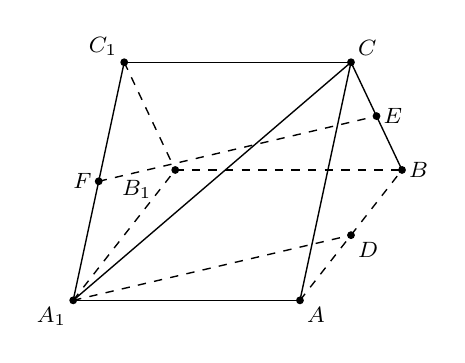
\begin{tikzpicture}[font=\footnotesize, line width=0.5pt, scale=0.72,
  dot/.style={circle, fill=black, inner sep=1.0pt}]
  \coordinate (A1) at (0,0);
  \coordinate (A)  at (4,0);
  \coordinate (C1) at (0.9,4.2);
  \coordinate (C)  at (4.9,4.2);
  \coordinate (B)  at (5.8,2.3);
  \coordinate (B1) at (1.8,2.3);
  \coordinate (D)  at (4.9,1.15);
  \coordinate (E)  at (5.35,3.25);
  \coordinate (F)  at (0.45,2.1);
  % 可见棱与可见面上的辅助线
  \draw (A1) -- (A);
  \draw (A) -- (C);
  \draw (C) -- (C1);
  \draw (C1) -- (A1);
  \draw (C) -- (B);
  \draw (A1) -- (C);
  % 不可见棱与内部辅助线
  \draw[dashed] (A) -- (B);
  \draw[dashed] (B1) -- (B);
  \draw[dashed] (C1) -- (B1);
  \draw[dashed] (A1) -- (B1);
  \draw[dashed] (A1) -- (D);
  \draw[dashed] (F) -- (E);
  \foreach \p in {A,B,C,A1,B1,C1,D,E,F} \node[dot] at (\p) {};
  \node[above left=-1pt] at (C1) {$C_1$};
  \node[above right=-1pt] at (C) {$C$};
  \node[below left=-1pt] at (A1) {$A_1$};
  \node[below right=-1pt] at (A) {$A$};
  \node[right=-1pt] at (B) {$B$};
  \node[left=5pt, yshift=-7pt] at (B1) {$B_1$};
  \node[below right=-1pt] at (D) {$D$};
  \node[right=-1pt] at (E) {$E$};
  \node[left=-1pt] at (F) {$F$};
\end{tikzpicture}
\end{center}
\nopagebreak[4]
\end{question}
\begin{question}
\gkti{18}设椭圆 $\dfrac{x^2}{a^2}+\dfrac{y^2}{b^2}=1$（$a>b>0$）的左焦点为 $F$，离心率为 $\dfrac{\sqrt3}3$，过点 $F$ 且与 $x$ 轴垂直的直线被椭圆截得的线段长为 $\dfrac{4\sqrt3}3$。

（1） 求椭圆的方程；

（2） 设 $A$，$B$ 分别为椭圆的左、右顶点，过点 $F$ 且斜率为 $k$ 的直线与椭圆交于 $C$，$D$ 两点。若 $\overrightarrow{AC}\cdot\overrightarrow{DB}+\overrightarrow{AD}\cdot\overrightarrow{CB}=8$，求 $k$ 的值。

\end{question}
\begin{question}
\gkti{19}已知首项为 $\dfrac32$ 的等比数列 $\{a_n\}$ 的前 $n$ 项和为 $S_n$（$n\in\mathbf N^*$），且 $-2S_2$，$S_3$，$4S_4$ 成等差数列。

（1） 求数列 $\{a_n\}$ 的通项公式；

（2） 证明 $S_n+\dfrac1{S_n}\leqslant\dfrac{13}6$（$n\in\mathbf N^*$）。

\end{question}
\begin{question}
\gkti{20}设 $a\in[-2,0]$，已知函数 $f(x)=\begin{cases}x^3-(a+5)x, & x\leqslant0,\\ x^3-\dfrac{a+3}2x^2+ax, & x>0.\end{cases}$

（1） 证明：$f(x)$ 在区间 $(-1,1)$ 内单调递减，在区间 $(1,+\infty)$ 内单调递增；

（2） 设曲线 $y=f(x)$ 在点 $P_i(x_i,f(x_i))$（$i=1$，$2$，$3$）处的切线相互平行，且 $x_1x_2x_3\neq0$，证明：$x_1+x_2+x_3>-\dfrac13$。

\end{question}